\setcounter{page}{1} \pagenumbering{arabic}
\chapter{Introduction}

This monograph presents theoretical and empirical considerations in the field of entrepreneurship. The fundamental idea is that the act of entrepreneurship expresses a crucial development of the social division of labour, a phenomena that already dates within the economics literature from the 18th century. We specifically recall the work of Adam Smith. Although Smith focusses on economic activities in society from a dynamic point of view his concept of the \emph{invisible hand}---and the notion that an economy is normally in some naturally \emph{stable state}---has dominated theoretical discourse within the economics discipline. Indeed, over the last two centuries the dynamic concept of economic interaction that Smith sought to discuss in the \emph{Wealth of Nations} has been substituted for more static analysis. This is reflected in general equilibrium analysis, a cornerstone of traditional economic theory. The result of this analysis states that if there exists no government interference with the economic activities of the agents in society, then these individual activities bring about a stable situation, which can be valued as a natural equilibrium in the economy. The work of Smith does not just deal with this issue, but develops a philosophical and ethical framework to comprehend all economic activities in a society~\citep{Gilles1990}.

% The idea of the invisible hand has been repelled as well as taken as a starting point in the design of some economic theory. 

The arrival of an economic system to a well-defined equilibrium steady state seems to contradict the notion of active entrepreneurship. We note that the act of entrepreneurship is a dynamic, disruptive force that cannot emerge from a static steady state defined by general equilibrium theory\footnote{This is a perspective that this shared with heterodox economic writers, such as~\citet{Schumpeter1942}}. As a consequence the notion of an entrepreneur and the act of entrepreneurship is ill-defined in traditional economic theory. The most compelling definitions of entrepreneurship emerge within more heterodox strands of the economics and sociology literature and, as a consequence, lacks an elaborate theoretical basis. The outcome is a shallow insight into the environmental context of entrepreneurship and the result that entrepreneurship has on the organisation and distribution of power within society.

The theory as developed in this monograph is based on the assumption that the institutional structure and organisation of the trade processes in the economy is crucial. This monograph values the general equilibrium concept as an expression of a specific and efficient form of organisation of the trade processes in the economy. Indeed, the assumptions enforced by the Walrasian general equilibrium model lead to the formation of a market whereby the axiom of perfectly competitive behaviour of agents is expressed. The institutional structure is inflexible and the resulting organisation of society is perfectly formed. A more general way to consider the organisation of trade processes is that of a network, which emerges as a consequence of a pattern of exchanges between agents of a society under a given mechanism of trade. Under the Walrasian model of general equilibrium a complete network emerges representing perfectly efficient market processes. In reality networked markets are imperfectly connected; there exist structural holes and opportunities for brokerage. Further, instead of the Walrasian general equilibrium theory to be reflective of the fundamental idea of the invisible hand, as is typically claimed, we note that it is the organisation of society with respect to the networks and institutions that guides the division of labour, the connectivity of society, and thus price levels.

Throughout this monograph we propose other forms of organisation of trade processes in the economy such as markets with imperfect structure, costly interactions, and heterogeneous positions of economic agents. In our view this provides a better description of the economic processes that takes place in reality. Moreover, we establish the theory of the economy as fundamentally dynamic, thus allowing for the development of entrepreneurship in a natural way. This is the purpose of our initial theorising regarding how we perceive the interaction space of the economy: to allow us to appropriately define the entrepreneur and act of entrepreneurship. From this we can analyse entrepreneurial action and power within the context of empirical examples.

The monograph consists of three parts each discussing certain modelling aspects of the economy, forms of trade organisation and entrepreneurial activity. In this chapter we introduce the notion of a socially structured economy and a background into the theory on social and economic interactions.

\section{Socially structured economies}

Economic theory is founded on the basis of \emph{methodological individualism}, \emph{methodological instrumentalism}, and \emph{equilibration}. With methodological individualism the decision-making agent has a central position in the theory. In most cases an economy is described as a configuration of such individual economic agents, who try to optimise some well-defined pre-determined goal or objective. In this configuration it is assumed that the economic agent possesses the tools to optimise their utility; this is the methodological instrumentalism of economic modelling \citep{Arnsperger2006}. This implies that economic decision processes in the economy are determined by the individual decision behaviour of these economic agents and by the configuration in which these economic agents are located. The outcome of this interaction is an equilibrium state represented as an organisational steady state. The economic system transitions from one steady state to another through some exogenous shock; suggesting that any dynamism is purely transitory and whose roots are ill-defined.

An additional assumption is that the individual economic agent can be described completely with the use of individual attributes only. Examples of these individual attributes are an endowment bundle of commodities, individual production capacities, and an individual preference relation on the set of well-defined, achievable commodity bundles for the particular economic agent. An illustration of this important reliance on methodological individualism is with respect to the traditional Arrow-Debreu model of a perfectly competitive market system. This model contains a population of individual economic agents partitioned into a class of consumers and a class of producers. Consumers attempt to optimise a certain individual preference relation over the collection of achievable commodity bundles, while producers try to maximise their profit given their individual production capacities. These economic agents are placed within the context of a system of perfectly competitive markets, which puts certain constraints on the abilities of agents. The major constraint is given by the price levels determined by the market. Consumers limit themselves in terms of budget sets and, while producers adapt their production plan to maximise their profits. There is no consideration for other socially constructed characteristics that have an influence on the preferences and abilities of the individual decision-maker: the price level is the only `social' aspect that has a considerable influence on the population of individuals.

Within this context the application of methodological individualism is very specific. Only individual decision makers are participating in the processes that take place within the economy. Its use suggests that agents are essentially individuals, who are interacting with each other according to the rules of the economic organisation, and not with each other as a primitive social characteristic in their behaviour. This illustrates that this method of microeconomic theorising implicitly involves a certain requirement on the `rules of the game'. 

In this monograph we recognise that the rules of the game---which are representative of the social structure of the economy---are crucial in the design of a descriptive model of trade processes in that economy. Therefore, economic agents are not just individual decision makers, but decision makers within a certain organisational environment, in which this organisational environment is consisting of a social structure of the economy and certain behaviouristic rules of the game. The agent is therefore still considered to be a decision maker with some individual objective goal, but also explicitly considered within some organisational environment determined by a well-defined governance system. The fact that an agent is considered as embedded within an organisational environment, leads to the acceptance of certain so-called \emph{social constraints} on the behaviour of that economic agent. Furthermore, the agents activity is contained within a matrix of interactions thus suggesting that the structure of interactions can also impose a constraint to their decision-making.

We further note two additional implicit assumptions of traditional modelling. The first is that there exists a dichotomy between consumers and producers. The population of economic agents is partitioned into two non-intersecting sets, which interact between but not within one another. This assumption is relaxed in this monograph during our characterisation of the economic agent. The second refers to the structure of the producers production possibilities, which do not lend themselves to Smith's notion of increasing returns to specialisation. As a consequence specialised producers and professions do not emerge naturally within the Walrasian framework. In modelling economic agents we allow for increasing returns to specialisation through learning, which stands in contrast to the Arrow-Debreu model and other general equilibrium models based on its foundation.

% summary of AD model

\medskip\noindent \citet[p.~5]{Gilles1990} notes that the Arrow-Debreu model shows that objective market price expresses a specific form of aggregation---\emph{Walrasian aggregation}---which is a hypothesis of the organisation as represented by the market. Within the model, the price is representing the aggregation of demand and supply within the organisation of a perfectly competitive market. As a consequence, all agents communicate with each other through the market price only, and not with each other directly. \citet{GillesDiamantaras2003} notes that this leads to a puzzle based on cyclical logic. But it more fundamentally suggests the inflexibility of perfect competition as an extremely efficient market structure. It is based on individualistic and symmetric economic agents that react to signals from market prices. The result is an equilibrium with no endogenous deviation. Further, there are no deeper social features and attributes that influence the behaviour of the agents which shows that the functioning of the market is not influences by other factors other than the market price.

The Arrow-Debreu model expresses a socially structured economy, albeit in a limited sense. The interactions of a finite set of individualistic decision-makers generates an idealistic market characterised by an objective price level for the exchange of a good. We claim that this social structure is limited in the sense that it results in a static market mechanism shorn of all other social influences. In the real world prices are not objective as in Arrow-Debreu style general equilibrium modelling. The notion of perfect competition is purely \emph{idealised}. Market imperfections, bounded human rationality, institutional structures, and incomplete network architectures explain disparity and subjectivity in price levels. \citet{Blume2009} provide a model of exchange on a network based on the notion of Nash equilibrium. The model suggests that agents possessing dominant positions within a network of relations can influence price levels exposed to both producers and consumers. Models of this nature are discussed in Section~\ref{sec:socialeconomicnetworks} below. Institutions and socially constructed customs and cultures inform preferences and thus price levels within markets. We embrace these fundamentally social aspects of markets within our modelling.

\subsection{Objectives}

This discussion allows us to establish some objectives for the development of the monograph, within which we provide a theory regarding entrepreneurship and socially structured economies. Our first objective is to develop a perspective of embedded economic activity based on specialised economic agents that form a functional social division of labour. The deepening of the social division of labour leads to a generation of wealth that can benefit society as a whole. Specifically, we take a \emph{relational perspective} in which to view the foundations of social and economic phenomena. This foundation, established in Chapter~\ref{ch:relationalperspective}, provides a theory of social and economic interaction based on the use of socially embedded systems of governance which are successfully utilised given a foundation of trust. Notably, the relational perspective discussed embraces Smith, yet deviates substantially from traditional paradigm of the economics discipline founded on the Arrow-Debreu model.

The second objective is to explain and illustrate the role of the entrepreneur within the relational perspective and highlight the impact that entrepreneurship has on the evolution of the social division of labour, and therefore the development or, in some instances, the regression of the economy. Within our theory we note that the entrepreneur can have an impact on different layers of the economy: specifically impacting economic agents themselves, the economic interaction networks, and the institutions of the interaction environment. To this we apply our theory of the entrepreneur to empirical case studies.

The third objective is to provide a distinction between the act of entrepreneurship and the entrepreneurial function of the economy. The latter relates to the adaptive and creative act that many economic agents perform in producing outputs; this facilitates differentiation and great economic wealth, but not necessarily a new species of work or profession. The former relates to incredibly creative and disruptive acts that are reflective in the organisation of society and the interaction of new specialisations.

A final objective is to complement our theoretical discussion of the relational perspective and entrepreneurship with empirical analysis of entrepreneurial activities. This involves creating a set of tools that allows us to analyse data in a pragmatic way. From these tools we can identify influential positions and activities within a networked economy.

% Although there has been discussion within the recent economic and sociological literature with regards a movement towards a relational perspective of the economy, none of the proposed theories have provided a convincing foundation in which to build upon. Many lack precise definitions to the notions and concepts they use, and most of which are still very much ingrained in traditional market theory. Importantly, none of the theories provide any insight or mechanisms in which to model and perceive the dynamic evolution of the relational social and economic environment through an institutional or entrepreneurial force. These models are still largely based on the foundation of equilibrium analysis, and thus do not provide any insight into the dynamics of economies. Moreover, despite much discussion within academic economics with regards issues of "networks" and "trust", and recent policies targeted towards the requirement of "entrepreneurs" to bolster economic prosperity, there still remains a lack of consensus in how to perceive these difficult notions.

\medskip\noindent To develop an evolutionary theory, as portrayed by the relational perspective, we must first provide a detailed insight into our fundamental units of analysis: the human agent and society, which is at the basis of all socio-economic activity. In the first section of developing the relational perspective we investigate the micro-foundational elements of the human agent; elaborating on the agents innate ability to form social relationships with each other. The human brain has co-evolved with the growth of the increasingly complex social environment that we have had to navigate and coordinate. We align our analysis with the hypothesis that the human brain has not developed in order to understand informational attributes of our environment but, converse to the conventional wisdom, our brains still remain imperfect in understanding objective information about the world. The economic decisions we make in complex situations are only made on the basis of bounded rationality, with informational constraints, and in situations of uncertainty. Moreover, our subjective perspectives and preferences can be manipulated by the opinions and norms embedded within our own socio-economic network.

From this perspective of the human actor, and the society in which she is embedded, we elaborate on a theory that takes an architectural analysis of social and economic interactions through the evolution of institution that facilitates exchange and deepening of the division of labour. We suggest that the division of labour naturally leads to the formation of relational networks, and from this we investigate the evolution of these relational networks---and thus the evolution of the economy---through the perspective of the entrepreneurial function primarily as an extension of the division of labour. So, we contend that the evolution of the socio-economic networks, and the systems of governance that hold them together, can only be explained through the use of the entrepreneurial function and the consequential extension, or contraction, of the social division of labour.

% In short, the RP is a microeconomic theory with macroeconomic implications. From the fundamental notion of socially embedded economic interactions \citep{Granovetter1985, Granovetter2005} we hope to provide the basis of economic development using complimentary institutional and entrepreneurial aspects that facilitate change and growth. This perspective is in line with \citet{Schumpeter1942} in suggesting that it is the entrepreneurial function of the economy that drives Creative Destruction through innovation which subsequently leads to macroeconomic change. Moreover, the perspective is in line with New Institutional Economists and theorists in Evolutionary Economics who accept that institutional mechanisms tend to operate in a 'meso' domain of the economy and are reflected by microeconomic actions and subsequently also affect macroeconomic outcomes of a specific economy \citep{dopfer2004}. Specifically, socio-economic institutions operate in between the micro and macro domains of the economy and have simultaneous causality with them both. We suggest the entrepreneurial actions have the potential to influence the institutional context of the economy and thus drive macroeconomic development.

\subsection{Motivation}

The pursuit to develop a novel model for investigating socio-economic phenomena has come from two overlapping concerns. The first concern is prompted from the apparent deficiency in mainstream theory to convincingly address the emergence of new organisational structures and technologies and to fully incorporate the entrepreneurial function within the economy. The entrepreneur is left undeveloped in many formal economic theories. The main problem of these mainstream theories in appropriately modelling the entrepreneurial function derives from the use of specific Walrasian axioms based on the notion of general equilibrium as expressed above. Economic markets tend to converge to a predetermined equilibrium state whereby unique market-clearing prices for homogeneous outputs emerge. At such a point it is difficult to endogenously integrate the development of an innovative technology into the model without having to assume its eventual existence which exogenously disrupts the growth of the economy. Well-established endogenous growth models have been created to formally explain how the generation of ideas from a research sector can lead to economic growth~\citep{Romer1990}, however these models do not truly integrate differentiated and innovative commodities, nor do they specifically integrate the entrepreneur. In order to integrate the entrepreneurial function it may be beneficial to maintain that the notion of static equilibrium is a purely intellectual concept that, in reality, fails to emerge. Much like the Austrian perspective on the matter, opportunities arise when the economy is out of equilibrium; and much like the Schumpeterian perspective, the entrepreneurs actions actively \emph{disequilibriate} the economy thus facilitating the emergence of increasingly more opportunities and innovation to take place meaning that equilibrium will never emerge. Thus, we should advocate that the economy has the potential to be in a continual state of dynamism.

Second, and perhaps more importantly, there seems to be an underlying disgruntlement within the economics discipline which has especially come to light in both academic and popular literature since the Global Financial Crisis of 2008. Some economists believe that the fundamental problem derives from the fact that the economics discipline has become progressively divorced from economic reality.~\citet{Hodgson2009},~\citet{Smith2010}, and~\citet{Keen2011} have appealed for a complete reform of the economics discipline as opposed to continually building increasingly esoteric and irrelevant mathematical models on top of a broken paradigm. These critics typically agree that the focus of the discipline has to change from it's overwhelming focus on elegant General Equilibrium models that provide highly trivial results to a more pragmatic and empirically founded approach based on inductive reasoning. Where the discipline should concentrate its efforts remains debatable and highly sensitive to the subjective opinion of the academic economist. We agree with Hodgson that, in order to be pragmatic, we must orient ourselves to understanding real-world institutional environments and actors. However, it is important to initially be more fundamental than that; we must first understand the mechanisms concerning the embeddedness of economic activity in social constructs, the implications of the resulting division of labour and trade, and the development of innovation which is at the heart of the entrepreneurial function.

The disgruntlement concerning the economics discipline is far from new. Previous Nobel Prize winners, such as Wassily Leontief, Milton Friedman, and John Hicks have expressed their concern. Ronald \citet{Coase1997} was explicit in claiming that, ``[e]xisting economics is a theoretical system which floats in the air and which bears little relation to what happens in the real world... I would say it has no subject matter. That's the problem.'' \citet{Knight1921} opened his influential book, \textit{Risk, Uncertainty, and Profit}, by highlighting the problems of theoretical economics perceiving itself as the only social science aspiring to become an exact science. He suggests that we have provided ourselves with a seemingly impossible task of identifying, and anatomising extremely complicated and intertwined social and economic phenomena, which perhaps cannot be measured. Even at that time Knight highlighted the problems of divorcing a single individual from the entirety of the structure the interact in. Moreover, \citet{Krugman2009}, \citet{Stiglitz2010}, and \citet{Varoufakis2011} have expressed their concerns regarding the disciplines divorce from reality and it's politically-driven ideology. The discipline may be better categorised as a subjective art---or even in some cases as a religion---as opposed to a true and exact science \citep{Backhouse2010}.

% Although quick to criticise the academic pursuits of the economics discipline since the recent financial crisis, no economist has provided a convincing theory in which to frame social and economic activities, and thus explain development and prosperity. Importantly, no economist has provided fundamental notions on which to build upon in order to explain economic interaction and development. New Institutional Economics (NIE) still provides the most promising branch of theory in which to provide useful policies for both firms and State. But the theories put forward are stubbornly superficial to aspects of the division of labour, increasing returns, the composition of society, and the social relations that underpin the economic activities. Indeed, NIE seems to be bereft of one of the most important institutions of all: civil society. Arguably, these features are initially mentioned by pioneering New Institutional Economists such as \citet{North1989, North1990}, however they have not been given the full discussion they deserve. Indeed, any general theory or elaborate discussion that has been provided by North is typically disjunctured and unconvincing.

\medskip \noindent This monograph provides the foundations of a coherent and productive paradigm; a holistic perspective in which to frame social and economic phenomena. The relational perspective that is advocated revolves around a number of interdependent microeconomic concepts: institutions, increasing returns to specialisation, the division of labour, and entrepreneurship. Using the foundational concepts of the relational perspective we explain the entrepreneur and the entrepreneurial function within the economy, therefore investigating innovation and the emergence of new institutional and organisational structures.

This discussion of the entrepreneur is not one that considers a single economic agent exogenously endowed with entrepreneurial talent or ability within a social and institutional vacuum as is considered in much of psychology. The perception of the entrepreneur in this monograph is a story of economic institutions, social structure, and the positions and actions of individuals within society. Through the analysis of this revolutionary character we can also tell a story of dynamic change within both the technological and institutional spheres of the economy, as well as a story on the current state of the institutions that facilitate and guide the entrepreneur and the division of labour, and how they may be improved to allow for progressive social and economic development.

% The rest of the chapter will investigate the state of the economics discipline with respect to the entrepreneur and the entrepreneurial function. After the discussion regarding the current state of the entrepreneur we claim that the apparent problems of modelling the entrepreneur within neo-classical economics stem from its neo-Walrasian foundations. Subsequently we provide an in-depth discussion of the realism of the fundamental axioms of the neo-Walrasian paradigm, which motivates our insight into the RP in which to view microeconomic phenomena and the entrepreneur.

% The RP will be discussed in more elaborate detail in chapter 2, and the evolutionary extension which considers the entrepreneurial function will be investigated in greater detail in chapter 3. Providing foundation of the RP allows us to model the topology and evolution of networks and also allows us to answer the important questions surrounding the entrepreneur and the emergence of new divisions of labour that support the functioning of new institutional mechanisms and technologies. Indeed, only after I have provided an overview of issues such as trust, governance, and the the division of labour, am I really in a position to provide a comprehensive definition of the entrepreneur.

\section{The relational perspective}

All economic activity is socially embedded. As such, economic agents are innately social. We wish to introduce these social characteristics into the description of the economic agent. This is done in a direct manner such that we describe social characteristics as potential pairwise relationships between economic agents, that are relevant with respect to the economic actions of these agents. The most natural of these relationships is a potential economic exchange relationship; two agents, who are related in a fundamentally social way, may activate their trade relation if it is mutually beneficial to do so.

The introduction of these social characteristics, in the form of pairwise relationships, leads to the formation of a global social structure on the population of economic agents. These social characteristics are specifically not individualised but should instead be seen as relational in that they must involve more than one economic agent to exist. In following~\citep{Gilles1990} we note that the relations between economic agents can be treated separately from the individual characteristics of those agents. The application of this modelling principle allows us to talk about the network of relations independently from the characteristics of the agent. As such, we apply graph theory to the analysis of the relational perspective. An introduction to the theoretical and empirical debates on social and economic networks are given in Section~\ref{sec:socialeconomicnetworks} below.

The evolving relational structure places social constraints on each individual economic agent. These social constraints come from two phenomena. First, from the relational structure of social and economic networks that the agents develop through social relationships and exchange. Second, from the socially constructed institutions and systems of governance that guide agents through the formation of relational networks. The existence of systems of governance brings with it a rule set that constrains the potential actions of individual agents and allocates resources between the population of economic agents. Both social constraints are investigated throughout the monograph.

The analysis into social structure and social constraints is not new. The investigation to how participants act within a social economy was one of the eventual objectives of~\citet{vNM}. This general research into the interaction of social structure and economic outcomes was extended by~\citet{KalaiMiddlemen1978} who remarked that social defects within an economic environment can lead to an uneven distribution of power within society. Specifically, there will exist an unequal distribution of power throughout society. Indeed, intermediating agents can potentially leverage their position within a matrix of relationships, exercising their power on others agents that they are connected to. An interesting point is raised---and one that is noted in other works since \citet{Granovetter2005}---is that the social abilities of a set of agents can have a significant impact on their economic outcomes\footnote{It is worth noting that although the economic benefits of dominant middleman activities have been substantially highlighted, \citet{KalaiMiddlemen1978} focus also on the costly disadvantages of sustaining a middleman position. Specifically, through a comparison of the Core, the authors note that the position of a middleman can be burdensome.}.

\subsection{Middlemen and entrepreneurs}

The notion of a middleman is introduced in conjunction with that of a network. We define a middleman as a graph-theoretical concept and embed the notion of power---in terms of social and economic connectivity---within the context of \emph{centrality}. The philosophy behind this is to provide an objective measurement to economic power within an trading platform given some social structure. From this we can derive the distribution of utility through the network of socio-economic relationships. Indeed, the naturally forming network configuration represents the aggregate utility and the distribution of utility throughout society. These networked economies and the presence of middlemen can only be explained fully within a relational perspective of socio-economic activity.

This monograph combines the notion of a middleman with that of the entrepreneur. Specifically, we claim that the middleman position of an economic agent represents the existence of an entrepreneurial activity that has lead to a new specialisation, and thus an extension of the division of labour. The formation of a middleman position---whether it be through individual efforts or group activity---is illustrative of entrepreneurship and reflective of a changing interaction infrastructure.

We use numerous methodologies to analyse entrepreneurship and power within the relational perspective including graph theory, \emph{non-cooperative} game theory, and statistical analysis. Specifically, we use graph theory in identifying middleman and providing an objective measurement of power; non-cooperative game theoretic concepts to explain the formation of middleman positions within networked systems; and statistical analysis to measure the significance of an agents middleman position and centrality to their economic performance. This investigation into the notion of the middleman, and its relationship with the entrepreneur, is done after first establishing the relational perspective.

\section{An introduction to social and economic networks}
\label{sec:socialeconomicnetworks}

Much of the formal analysis of the relational perspective is based on network theory. This section provides initial definitions and insights into network theory and the literature around social and economic networks. Although some of this provides only a background to network analysis, many of the concepts discussed below are used more formally in subsequent chapters.

\subsection{Basic concepts}

A network is a graph with non-trivial topological features such that there exists a set of \emph{nodes}---which represent a corresponding set of social actors or economic agents---that are connected to one another in some fashion by a set of \emph{links}---that represent relationships---whereby each link can connect nodes either directly or indirectly. Nodes can be connected to each other by a \emph{path} if from one node to another there exists a set of links that can be traversed such that one node can manoeuvre to the other. The shortest path between any pair of nodes is termed as a \emph{geodesic path}, and the number of links that need to be traversed along this geodesic path is termed as the \emph{geodesic distance}. A \emph{strongly connected network} is one in which all nodes can connect to each other either directly or indirectly by a path.

Generally, it's found that many networked structures that emerge have topological properties that are neither purely random nor regular. Research into neural networks has highlighted a commonality regarding the complexity and networked structure of seemingly unrelated social, economic, and natural systems \citep{SpornsTononi2005, Sporns2010}. When modelling the structure of social networks \citet[p.~440]{WattsStrogatz1998} noted that, ``these systems can be highly clustered, like regular lattices, yet have small characteristic path lengths, like random graphs''. Many complex networks exhibit this mixture between random and non-random wiring whereby a few small dense clusters of actors are connected together by a few weak relationships.

A scale-free network, formally developed by \citet{BarabasiAlbert1999}, is one in which the number of links that an actor has in the network is unequally distributed such that there exists a minority of actors with many links and a majority of actors with relatively few links. Actors with relatively many links are termed as \emph{hubs}; the presence of hubs substantially reduces the diameter of the network.

\subsection{Characteristics of social networks}

\citet{JacksonRogers2007} summarise some key empirical regularities shared by networks created by social actors. First, they note that the average geodesic distance between any pair of nodes in the network has a tendency to be small, which corresponds well with the above finding of densification, and the maximum distance between any pair of nodes in a social network is small. This observation that there may exist a short distance between any two individuals, or nodes, was initially noted by Hungarian playwright Frigyes \citet{Karinthy1929} who conducted a thought-experiment regarding how close two random people were to each other by their local connections. Also, sociologist Georg Simmel described modern society as consisting of loosely connected social circles of relationships \citep{Simmel1950}.

This thought-experiment was operationalised and later carried out in a more scientific way in the form of the \emph{small-world experiment} by Stanley \citet{Milgram1967}. This experiment was was based on the methodology whereby a letter sent from a city in the midwest of the USA to Boston, USA, by means of transfer between personal acquaintances. The small-world experiment was designed to measure these path lengths by developing a procedure to count the number of links between any two acquaintances in the corresponding chain. The experiment resulted in the fact that the average observed path length was between 5.5 and 6, resulting into the well-known phrase ``Six Degrees of Separation''. This experiment has been replicated across different countries and with different techniques and the general finding by Milgram has been maintained; thus there tends to exist a low distance between any pair of nodes relative to the size of the population as a whole.

Second, Jackson and Rogers note that the clustering coefficient of the network---which measures the tendency of connected nodes to have common neighbours---are larger in social networks compared to networks where the links are randomly generated between nodes. This finding suggests that communities are formed in the network whereby nodes who share a given personal, geographical, or institutional characteristic tends to form a link with each other \citep{Watts2002}. The aggregation of these links across a number of nodes forms a clique, such that all nodes within a cliques are connected to each other. \citet{KossinetsWatts2006} note that \emph{focal closure}---whereby people who are members of the same affiliation have a tendency to form a link with each other---as a reason for why we tend to see this clustered pattern of communities on a network. This finding is associated with the notion of social foci, developed by Scott \citet{Feld1981, Feld1982}, as organisations that induce high connectivity between members.

Third, the distribution of the number of links a node has, i.e., a nodes \emph{degree}, tends to exhibit fat tails so that there are more nodes with relatively high and low degrees and fewer nodes with medium degrees than one would find if the links were formed in a random way. The degree distribution can be claimed to be approximately \emph{scale-free} such that the distribution follows a power-law. People who are more popular in terms of the number of connections they have are seen to be more attractive to form a relationship with, thus inducing this rich-gets-richer phenomenon initially found by \citet{Simon1955}.

Fourth, there tends to exist some positive \emph{assortativity} such that the degrees of connected nodes tends to be positively correlated in that nodes with a large degree tend to be connected to other nodes with a large degree, and nodes with a low degree tend to be connected to each other \citep{Newman2003mixing}. This assortativity between nodes extends beyond topological properties of networks such that nodes with a certain personal characteristics form connections between each other; this is a notion, distinct from assortativity, is known as \emph{homophily}. These notions of assortativity and homophily are initial findings of the context of social networks in sociology \citep{McPherson2001}, and remain interesting topics in medicine and finance \citep{Haldane2009, HaldaneMay2011}.

Finally, Jackson and Rogers note that the clustering among neighbours of a given node tends to be inversely related to the nodes degree. This final point is highly intuitive---especially given the notion of positive assortativity between nodes in a network---as the probability of all of a well-connected nodes neighbours to be connected to each other would be low.

\subsubsection{Models of social networks}

Since noting these characteristics a variety of random graph models have been proposed to explain some of the characteristics. The three most common models are that of a \emph{random network}, a \emph{small-world network}, and a \emph{scale-free network}. The notable structures of small-world and scale-free networks can be seen in Figure~\ref{networks} (a) and (b) respectively. These models of network formation can be either random and algorithmic, or can be strategic with the use of game theory whereby individual agents have some incentive to either form or sever links.

\begin{figure}[t]
\label{networks}
\begin{center}
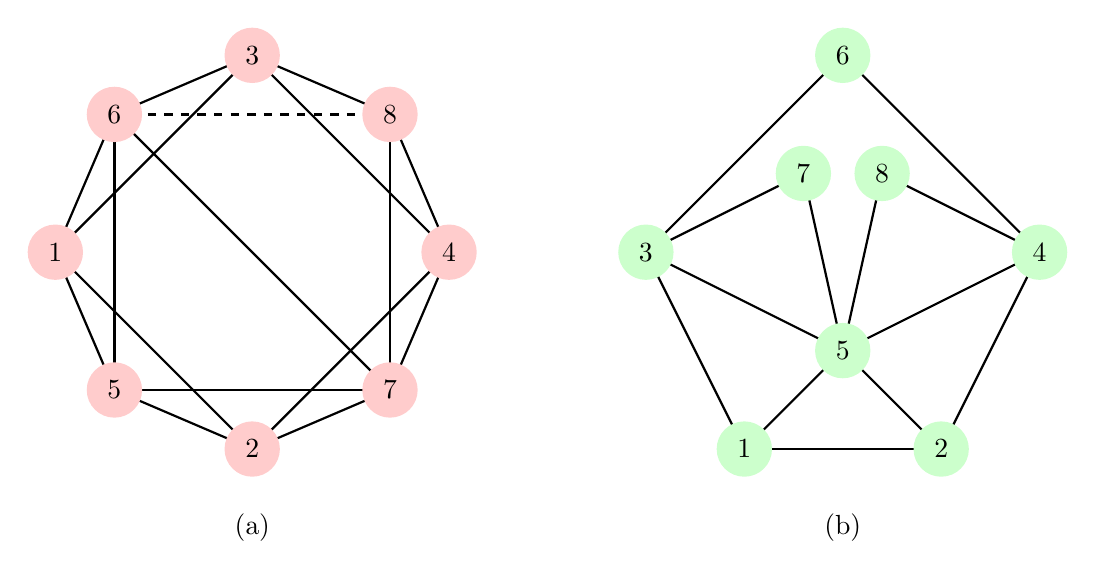
\begin{tikzpicture}[scale=0.5]
\draw[thick] (0,5) -- (5,0);
\draw[thick] (10,5) -- (5,0);
\draw[thick] (5,10) -- (10,5);
\draw[thick] (5,10) -- (0,5);
\draw[thick] (1.5,1.5) -- (1.5,8.5);
\draw[thick, dashed] (1.5,8.5) -- (8.5,8.5);
\draw[thick] (1.5,8.5) -- (8.5,1.5);
\draw[thick] (8.5,8.5) -- (8.5,1.5);
\draw[thick] (8.5,1.5) -- (1.5,1.5);
\draw[thick] (0,5) -- (1.5,1.5);
\draw[thick] (1.5,1.5) -- (5,0);
\draw[thick] (5,0) -- (8.5,1.5);
\draw[thick] (8.5,1.5) -- (10,5);
\draw[thick] (10,5) -- (8.5,8.5);
\draw[thick] (8.5,8.5) -- (5,10);
\draw[thick] (5,10) -- (1.5,8.5);
\draw[thick] (1.5,8.5) -- (0,5);

%\draw[thick] (1.5,1.5) -- (8.5,8.5);
%\draw[thick] (8.5,1.5) -- (0,5);
%\draw[thick] (8.5,1.5) -- (1.5,8.5);

\draw[thick] (17.5,0) -- (22.5,0);
\draw[thick] (17.5,0) -- (15,5);
\draw[thick] (17.5,0) -- (20,2.5);
\draw[thick] (22.5,0) -- (20,2.5);
\draw[thick] (22.5,0) -- (25,5);
\draw[thick] (25,5) -- (20,2.5);
\draw[thick] (25,5) -- (20,10);
\draw[thick] (25,5) -- (21,7);
\draw[thick] (20,2.5) -- (19,7);
\draw[thick] (20,2.5) -- (15,5);
\draw[thick] (15,5) -- (20,10);
\draw[thick] (20,2.5) -- (21,7);
\draw[thick] (19,7) -- (15,5);

\draw (0,5) node[minimum size=2em,circle,fill=red!20] {$1$};
\draw (5,0) node[minimum size=2em,circle,fill=red!20] {$2$};
\draw (5,10) node[minimum size=2em,circle,fill=red!20] {$3$};
\draw (10,5) node[minimum size=2em,circle,fill=red!20] {$4$};
\draw (1.5,1.5) node[minimum size=2em,circle,fill=red!20] {$5$};
\draw (1.5,8.5) node[minimum size=2em,circle,fill=red!20] {$6$};
\draw (8.5,1.5) node[minimum size=2em,circle,fill=red!20] {$7$};
\draw (8.5,8.5) node[minimum size=2em,circle,fill=red!20] {$8$};
\draw (17.5,0) node[minimum size=2em,circle,fill=green!20] {$1$};
\draw (22.5,0) node[minimum size=2em,circle,fill=green!20] {$2$};
\draw (15,5) node[minimum size=2em,circle,fill=green!20] {$3$};
\draw (25,5) node[minimum size=2em,circle,fill=green!20] {$4$};
\draw (20,2.5) node[minimum size=2em,circle,fill=green!20] {$5$};
\draw (20,10) node[minimum size=2em,circle,fill=green!20] {$6$};
\draw (19,7) node[minimum size=2em,circle,fill=green!20] {$7$};
\draw (21,7) node[minimum size=2em,circle,fill=green!20] {$8$};

\draw (5,-2) node {(a)};
\draw (20,-2) node {(b)};
\end{tikzpicture}
\end{center}
\caption[Small-world and scale-free networks]{Network (a) shows a circular small-world model and network (b) shows a scale-free model.}
\end{figure}

\paragraph{Random graph models.}

The first set of network formation models to be developed are based on the random generation of links between nodes. A random graph is the general term that refers to probability distributions over graphs. Random graphs may be described by a probability distribution, or by a random process which generates them. They are obtained by having an initial set of unconnected nodes and then randomly connecting nodes together by a set of links. The initial research into random graph models was conducted by \citet{ErdosRenyi1959}. The seminal model developed serves as the basis for all subsequent random graph models \citep{Gilbert1959, Bollobas2001}.

A number of properties are derived from the random graph models. An important property is that of a \emph{phase transition}. A phase transition refers to a punctuated change in the state, structure and dynamics of a complex system, that arises from a slight change in a variable that characterises the system as a whole. In the context of an Erd\"{o}s-R\'{e}nyi graph, if the probability of nodes being connected falls below a certain threshold the network will most certainly be \emph{disconnected}, such that there will exist at least one node that is not connected---at least indirectly---to other nodes and thus there cannot exist a strongly connected network. Above the threshold then the network will be strongly connected. The phase transition from a connected network to a disconnected network thus occurs when the probability of nodes being connected falls below a well-defined level.

Although theoretically compelling, many social and economic networks are not formed `randomly'. For example, empirical social networks are much more clustered than those generated by random. Real-world networks are neither completely ordered nor completely random, but rather exhibit important properties of both. Models of small-world networks add `order' to the network by assuming a regular lattice as the starting point.

\paragraph{Small-world networks.}

A small-world network is one whereby nodes are not necessarily neighbours of one another, but most nodes can be reached from every other by a small number of steps. In this form of network, \citet{WattsStrogatz1998}, \citet{Watts1999}, and \citet{NewmanStrogatzWatts2001} generate networks by starting with a symmetric, regular network and randomly rewiring some links between nodes. They found that the random rewiring process leads to an exponential decrease in the average distance between any two nodes whilst maintaining a network that is much more clustered than just randomly wiring the network. Figure~\ref{networks} (a) effectively shows the Watts-Strogatz model of small-world networks. In this example, a regular lattice is generated on a set of eight nodes whereby each node has four links each. Node 6 is rewired to another randomly, which reduces the average path length of the network.

\citet{Kleinberg2000a, Kleinberg2000b} also provides an algorithmic approach to modelling the small-world phenomenon in which he develops a decentralised algorithm to derive the efficient amount of randomness required to generate a small-world network. In the economics literature, \citet{JacksonRogers2005} provide game theoretic approach to the formation of pairwise stable small-world networks where agents wish to maximise the amount of information they have access to either directly or indirectly given that the information flowing through the network depreciates the longer the geodesic path from one node to another.

\paragraph{Scale-free networks.}

A scale-free network is one in which the number of links that an actor has in the network is unequally distributed such that there exists a minority of actors with many links and a majority of actors with relatively few links. Actors with relatively many links are hubs whose presence reduces the diameter of the network. Research by \citet{Price1976}, \citet{BarabasiAlbert1999}, and \citet{CooperFrieze2003} has shown that networks with power law degree distributions result if nodes form links through the process of \emph{preferential attachment} (i.e., new nodes link to existing nodes with probabilities proportional to the existing nodes' degrees). Power-law distributions have also been shown to result if new nodes copy the links of a randomly identified node \citep{Kleinberg1999, Kumar2000}, or if networks are designed to optimise tolerance \citep{Fabrikant2003}. A variation on preferential attachment where only some nodes are active at any time \citep{Klemm2002a} has been shown to also exhibit small world properties. Some network models that grow overtime have been shown to exhibit assortivity and scale-freeness, e.g., \citet{Callaway2001} and \citet{Krapivsky2002}.

Research has shown that many social and economic networks share a scale-free property \citep{Faloutsos1999, DorogovtsevMendes2003, Barabasi2009, Barabasi2012}. Also, biological and mechanical networks also share this structure \citep{Barabasi2011}. Scale-free networks have a number of desirable qualities including robustness to random attacks and small diameters \citep{AlbertJeongBarabasi1999, AlbertJeongBarabasi2000}. As a consequence scale-free networks are prone to collapse due to targeted attacks and contagious processes.

While the aforementioned models result in some of the empirical regularities of large social networks, none of them are consistent with all of characteristics above. The closest network formation process to cover all of these properties is indeed from \citet{JacksonRogers2007} whereby agents enter the network and initially form a network randomly, then form other links to nodes based on the initial connections' links. This formation process---a hybrid between random and strategic network formation---provides a structure that is most resembling to real social networks. However, it is still questionable as to whether the methods of generating these `social' networks are actually resembling the processes underlying most of the large networks that we actually observe.

For the moment we are only interested in the structure and the methods of forming networks. In Chapter~\ref{ch:relationaltheory} we consider the formation of exchange networks under an algorithmic process. We find that depending on the method of exchange between nodes the overall structure of the network and the average utility of the population changes. The generation of these networks serves as a basis for the algorithmic generation of economic relationships.

\subsection{Economic networks}

There are many studies of markets as networks \citep{RauchCasella2001}. \citet{Uzzi1996} provides one of the most influential investigations regarding the importance of social relationships in the New York City clothing industry. He focussed on the type of relationship between the clothing firms. Specifically, he categorised relationship as ``market'' or ``arm's length'', which included one-time social and economic interactions; and ``special'' or ``close'' interactions, which included many relationships with repeated interactions. Uzzi found that three main aspects were important for these relationships and interactions, these are: joint problem-solving; trust; and information transfer. From his analysis he found that firms with more clustered and intertwined social and economic relationships have a greater probability of survival. To Uzzi, social and economic embeddedness helps firms to survive and thrive. Also, the study found the importance and differences of market economic and close social relationships.

\citet{Weisbuch2000} and \citet{KirmanVriend2001} consider the Marseille Fish Market where market prices are not posted publicly. This allows prices to be maximally flexible: Each producer decides about her own prices; different consumers might be set different prices; and prices can vary over time. Priced are communicated privately and there is no bargaining in this market. A number of outcomes emerge. First, there is widespread loyalty to a single producer, while the minority of consumers purchase from multiple producers. The market seems promotes trust and reciprocity between consumers and producers. Specifically, consumers follow an adaptive updating rule, with a higher tendency to visit producers who have met their demands in the past. \citet{Vignes1993} and \citet{VignesEtienne2011} assess the network structure and the distribution of price levels throughout the market. The trade pattern that emerges has an interesting feature in that there is persistent price dispersion that fits with the networked structure of the market. The network tended to follow a scale-free structure.

\citet{Granovetter1973} famously considered the labour market a social network of references. As part of his Ph.D. thesis he investigated how people within a certain professional socio-economic class typically found information regarding new job opportunities. He identified that people tended to obtain the most relevant information about job availability from contacts in their social neighbourhood. Less intuitively, he found that the best information often came from acquaintances as opposed to close friends or family. Granovetter claimed that every person who forms social relationships holds a mixture of both \emph{strong} and \emph{weak} ties; where strong ties pertained to close friends and family members, and weak ties pertained to acquaintances. According to Granovetter the labour market operates as a social network where information regarding job opportunities are disseminated through the network. Weak ties, as opposed to strong ties, held less redundant and therefore more diverse information which an individual could exploit when attaining a job. Much in the same vein as Granovetter, \citet[p.~333]{Jackson2008} suggests that social networks of a firms' existing employees can also provide a good resource for searching for suitable employees, `` [a] firm may simply want to hire people similar to the employees it already has. Given the homophily in many social networks, a firm can take advantage of its existing workforce to find other people with similar characteristics.'' The outcome of the assessment is that the labour market that exists is more intricate than one characterised by traditional microeconomic analysis of labour economics.

The theory of weak and strong ties has been at the cornerstone of much of economic sociology since Granovetter's initial findings. The weakest, and therefore most valuable in terms of information, relations are \emph{bridge} relations. These were discussed in depth by \citet{Burt1992}, who suggested that individuals could exploit these bridge relationships through the attainment of new and diverse sets of information \citep{Burt2004}. As such, there exist `positions of power' within social networks and networked markets where some positions are more influential than other positions.

Exchange theory is concerned with how the structure of relationships among agents affects exchange between them \citep{CookWhitmeyer1992}. These exchanges could include economic interactions, trading of favours, communication of information, or other social interactions. Typically this research is based on dyadic interactions, but since the work of Robert \citet{Emerson1962, Emerson1972a, Emerson1972b, Emerson1976} networks have played an increasingly important role in exchange theory. In his work, Emerson considered network interactions to explain power and dependencies when considering exchange. This theory of networks played a role in Emerson's work because all economic exchange depended on the availability of outside options; therefore assuming a relatively competitive market in which economic relations could be made and severed without any friction. Under such a perspective, economic interaction cannot be viewed without the context of the complete network of all potential interactions and relationships. Again, much like Burt, network positions matter and asymmetries of power tends to be expected.

\subsubsection{Models of economic networks}

Emerson's work combined with the mathematical research of matching in bipartite graphs \citep{Hall1935} provided the basis for more research in bilateral trading models \citep{Corominas-Bosch1999, Corominas-Bosch2004}. Much like the implicit assumption of general equilibrium models, these models assume a dichotomy between the demand and supply within an economy. Therefore, all networks that emerge are simply between a set of nodes who produce the supply of the economy and a set of nodes who demand the produced goods. \citet{Blume2009} provide a convincing model of economic exchange on a networks. They also dichotomise the forces of demand and supply by introducing a set of `consumers' and a set of `producers' whereby a consumer can only engage in an economic exchange with a producer. Each economic exchange is represented as a link. As a consequence a bipartite network is formed whereby economic exchange occurs across the links between consumers and producers. The structure of their model follows that of \citet{KrantonMinehart2001} whereby, again, the forces of demand and supply are partitioned therefore forming two disjoint sets of consumers and producers. This bipartite set-up is also taken by \citet[Chapter~10]{Jackson2008}. Easley and Kleinberg find that this networked structure provides some nice properties, being able to show that society's welfare is maximised when prices develop to guide consumers to producers. Moreover, they find that, along with \citet{Kakade2004a, Kakade2004b}, a network provides a good basis for price dispersion as was seen in the Marseille fish market case.

\begin{figure}[t]
\label{fig:bipartiteexchange}
\begin{center}
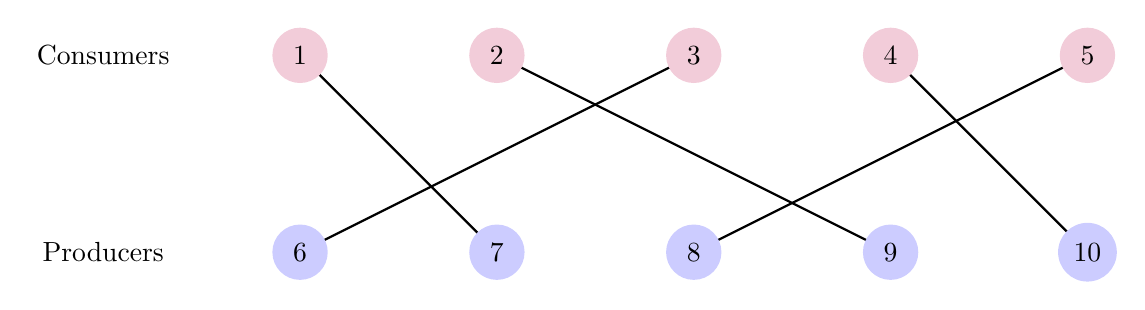
\begin{tikzpicture}[scale=0.5]
\draw[thick] (5,0) -- (15,5);
\draw[thick] (10,0) -- (5,5);
\draw[thick] (20,0) -- (10,5);
\draw[thick] (15,0) -- (25,5);
\draw[thick] (25,0) -- (20,5);

\draw (5,0) node[minimum size=2em,circle,fill=blue!20] {$6$};
\draw (5,5) node[minimum size=2em,circle,fill=purple!20] {$1$};

\draw (10,0) node[minimum size=2em,circle,fill=blue!20] {$7$};
\draw (10,5) node[minimum size=2em,circle,fill=purple!20] {$2$};

\draw (15,0) node[minimum size=2em,circle,fill=blue!20] {$8$};
\draw (15,5) node[minimum size=2em,circle,fill=purple!20] {$3$};

\draw (20,0) node[minimum size=2em,circle,fill=blue!20] {$9$};
\draw (20,5) node[minimum size=2em,circle,fill=purple!20] {$4$};

\draw (25,0) node[minimum size=2em,circle,fill=blue!20] {$10$};
\draw (25,5) node[minimum size=2em,circle,fill=purple!20] {$5$};

\draw (0,0) node {Producers};
\draw (0,5) node {Consumers};
\end{tikzpicture}
\end{center}
\caption{A matching market of consumers and producers}
\end{figure}

This bipartite representation of a market, known as a ``matching market'', can be seen in Figure~\ref{fig:bipartiteexchange}. This notion of a matching market is further extended by \citet{EasleyKleinberg2010} to include `traders' as intermediaries between consumers and producers. From this they informally define a notion of competition in a networked economy, suggesting that traders have an opportunity to monopolise flows of economic exchange between producers and consumers. The notion regarding the monopolisation of trade is extended and considered in detail in Chapters~\ref{ch:criticalnodes} and~\ref{ch:blocks} where we discuss measurements of brokerage in networked economies.

The reason why networks follow a bipartite structure is due to the way in which economic agents are characterised within the traditional perspective, and specifically the strict dichotomy between demand and supply~\footnote{When generating economic networks in Chapter~\ref{ch:relationaltheory} we do not assume the existence of a strict dichotomy between consumption and production and, as a direct consequence, a bipartite network does not typically emerge. Instead, when generating the exchange networks we arrive at properties that are more closely related to the typical structure of social networks as noted by the characteristics above.}. Within this monograph we note that economic agents are boundedly rational and exist within a network of social and economic relations that are influenced by systems of governance. However, the economic agent is further defined such that each individual is endowed with the powers of both production and consumption; that the forces of demand and supply are contained in all individual economic agents.

\section{Monograph structure}

This monograph is partitioned into three interlinked parts, each of which addresses the ultimate goal of developing a theory of the entrepreneur and entrepreneurial activity within a relational perspective of socio-economic activity. The first two parts are primarily focussed on theory, occasionally using empirical examples to illustrate and test models and measures. The final part is more focussed on explaining entrepreneurial activities within real-world case studies. Part~\ref{part:generalTheoryEntrepreneurship} consists of three chapters that provide a theoretical foundation to the relational perspective and an introduction to the entrepreneur. Much effort is spent developing the relational perspective framework, which is done from an evolutionary basis of the social actor that in turn represents an economic agent. Within this framework we are able to provide a holistic definition of the entrepreneur, linking the notion appropriately to the social division of labour and the networked structure that economic interaction produces. Of specific interest is the unique positions within the network that the entrepreneurial agent operates, and can be a source of their economic utility.

Part~\ref{part:entrepreneurshipPlatonianEconomy} consists of two chapters that elaborate on the interaction between entrepreneurship and the network interaction infrastructure. We investigate the establishment of uncontested middleman positions and the formation of blocks in relational economies. In elaborating on these concepts we develop formal models and measures to use on network-based data sets. These models and measures are then tested against the empirical data.

Part~\ref{part:entrepreneurshipPlatformEconomy}, the final Part of the monograph, also consists of two chapters that introduce an elaborate example of power within a more developed economy. This economic space is representative of a more layered economy within which there exist firms and directors that operate in multiple complementary industries. We analyse the directorial network and interlock formation in New York City from 1902--1912 as an entrepreneurial process. Indeed, these chapters investigate the establishment of power in New York City through network entrepreneurship and provide measures and models to investigate the centralisation of economic influence and use this to challenge claims regarding the history of the so-called \emph{Empire State} and the role of J.P. Morgan.
